% !TeX spellcheck = fr_FR
% !TeX encoding = ISO-8859-1

\section{Le 45�}

Ce point est particuli�rement important dans la mesure o� il constitue
une r�f�rence pour beaucoup de figures. Une fois acquis, il ne peut plus
�tre rat� (!). Il est facile. En cas d'�chec, notre ?il ou notre
position est responsable, voire notre distraction...

Il suffit de jouer en demi-bille la 2 du c�t� de la 3. � Prendre � une
demi-bille, c'est pousser la 1 en direction de la 2 de mani�re que, dans
son mouvement, la moiti� de la masse de la 1 co�ncide avec la moiti�
oppos�e de la masse de la 2... Pour une vis�e pr�cise, la 1 est prise au
centre bille, avec comme point de vis�e, la tangente � la 2. Il suffit
pour cela, une fois bien positionn�, de placer dans � sa vis�e �, le
bord de la 2 au milieu de l'image de la mouche de la fl�che.

Apr�s l'impact, la 1 ferait un angle de 45� si nous �tions dans un
espace � trois dimensions et sans frottement et si les billes 1 et 2
�taient en mouvement libre l'une vers l'autre et � vitesse �gale. Mais
comme nous sommes avec des volumes glissant sur un plan et qu'en plus le
mobile percuteur est en mouvement quand il s'�crase sur sa cible fixe et
... qui va se d�rober, l'angle est un peu inf�rieur, jusqu'� 40� si la
canne est tenue haute comme pour couler et jusqu'� 50� si la canne est
soutenue l�g�rement basse.

Retenons qu'une demi-bille a pour r�sultat un angle de 45�. Il y a une
erreur mais petite. En plus avec l'habitude, la merveilleuse m�canique
humaine va ajuster sans peine, ces petites diff�rences.

\begin{figure}[htb]
	\centering
	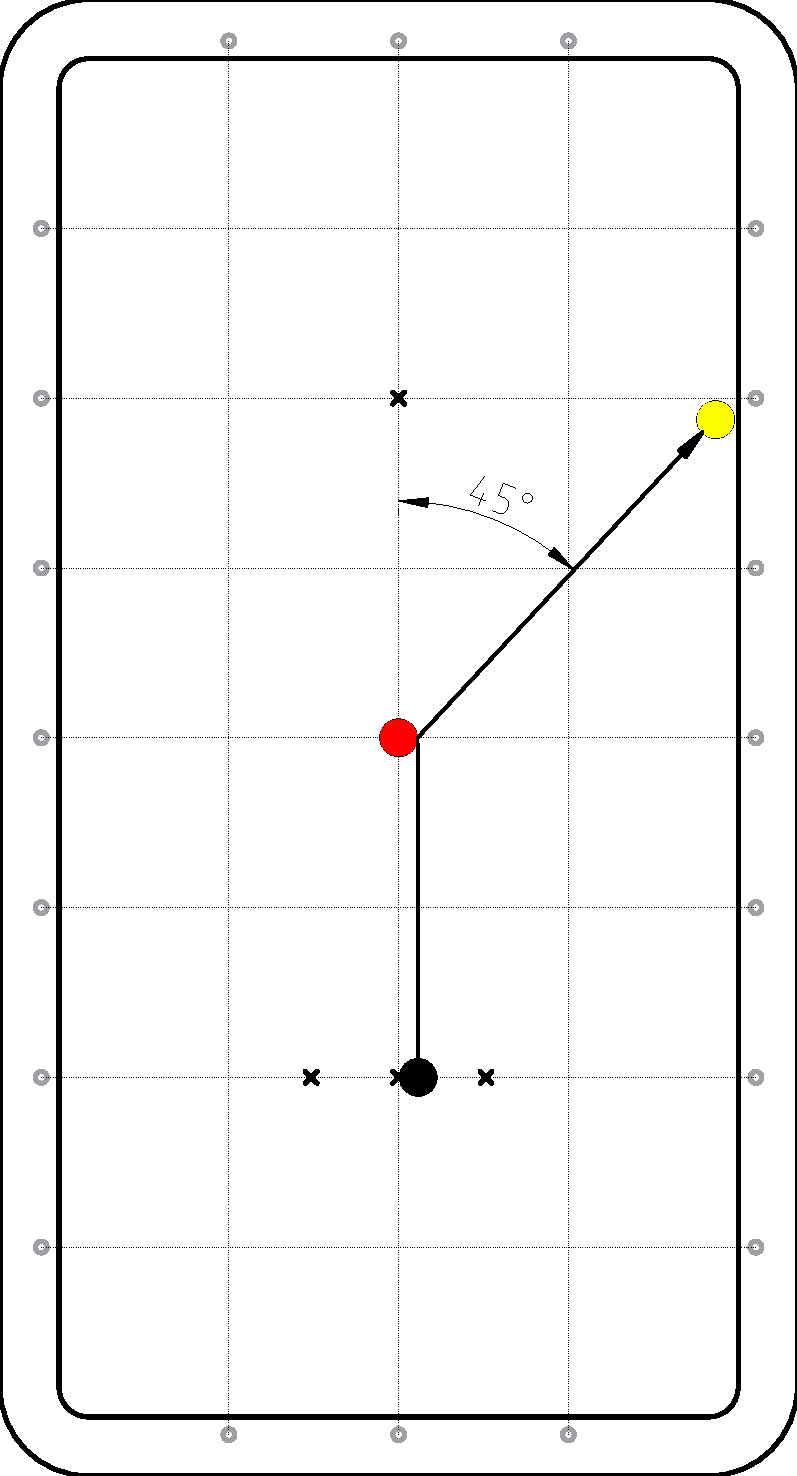
\includegraphics[width=0.85\linewidth]{A/imagesA/A07-1.pdf}
	\caption{Le 45�}
	\label{fig:a07-1}
\end{figure}
\clearpage
